 \let\negmedspace\undefined
\let\negthickspace\undefined
\documentclass[journal]{IEEEtran}
\usepackage[a5paper, margin=10mm, onecolumn]{geometry}
%\usepackage{lmodern} % Ensure lmodern is loaded for pdflatex
\usepackage{tfrupee} % Include tfrupee package

\setlength{\headheight}{1cm} % Set the height of the header box
\setlength{\headsep}{0mm}     % Set the distance between the header box and the top of the text
\usepackage{gvv-book}
\usepackage{gvv}
\usepackage{cite}
\usepackage{amsmath,amssymb,amsfonts,amsthm}
\usepackage{algorithmic}
\usepackage{graphicx}
\usepackage{textcomp}
\usepackage{xcolor}
\usepackage{txfonts}
\usepackage{listings}
\usepackage{enumitem}
\usepackage{mathtools}
\usepackage{gensymb}
\usepackage{comment}
\usepackage[breaklinks=true]{hyperref}
\usepackage{tkz-euclide} 
\usepackage{listings}
% \usepackage{gvv}                                        
\def\inputGnumericTable{}                                 
\usepackage[latin1]{inputenc}                                
\usepackage{color}                                            
\usepackage{array}                                            
\usepackage{longtable}                                       
\usepackage{calc}                                             
\usepackage{multirow}                                         
\usepackage{hhline}                                           
\usepackage{ifthen}                                           
\usepackage{lscape}



\usepackage{amsmath,amssymb}
\usepackage{booktabs}
\usepackage{tikz}
\usetikzlibrary{arrows.meta,angles,quotes}





\begin{document}

\bibliographystyle{IEEEtran}
\vspace{3cm}

\title{5.3.15}
\author{AI25BTECH11021 - Abhiram Reddy N}
% \maketitle
% \newpage
% \bigskip
{\let\newpage\relax\maketitle}

\renewcommand{\thefigure}{\theenumi}
\renewcommand{\thetable}{\theenumi}
\setlength{\intextsep}{10pt} % Space between text and floats


\numberwithin{equation}{enumi}
\numberwithin{figure}{enumi}
\renewcommand{\thetable}{\theenumi}


\section*{Question}
What type of lines will you get by drawing the graph of the pair of equations:
\[
x - 2y + 3 = 0 \quad \text{and} \quad 2x - 4y = 5\ ?
\]

\section*{Solution}

We will analyze the system using matrix and vector notation.

\subsection*{Step 1: Write both equations in standard form}

First, express both equations in the form:
\[
Ax + By = C
\]

Equation 1:
\begin{equation}
x - 2y = -3
\label{eq1}
\end{equation}

Equation 2:
\begin{equation}
2x - 4y = 5
\label{eq2}
\end{equation}

\subsection*{Step 2: Represent as matrices}

Let us write both equations in matrix form:
\begin{equation}
\mathbf{A} = \begin{bmatrix} 1 & -2 \\ 2 & -4 \end{bmatrix}, \quad
\mathbf{x} = \begin{bmatrix} x \\ y \end{bmatrix}, \quad
\mathbf{b} = \begin{bmatrix} -3 \\ 5 \end{bmatrix}
\end{equation}

Then the system is:
\begin{equation}
\mathbf{A} \mathbf{x} = \mathbf{b}
\end{equation}

\subsection*{Step 3: Check for consistency and dependency}

We analyze the coefficient matrix:
\[
\mathbf{A} = \begin{bmatrix} 1 & -2 \\ 2 & -4 \end{bmatrix}
\]

Observe that:
\begin{equation}
\text{Row 2} = 2 \times \text{Row 1}
\end{equation}

So, the equations are **linearly dependent** in coefficients. However, check the constants:
\[
\text{Equation 2 constant} = 5 \neq 2 \times (-3) = -6
\]

So the augmented matrix is:
\[
\left[\begin{array}{cc|c}
1 & -2 & -3 \\
2 & -4 & 5
\end{array}\right]
\]

Now,
\begin{equation}
\text{Rank of coefficient matrix } \mathbf{A} = 1, \quad
\text{Rank of augmented matrix} = 2
\end{equation}

\subsection*{Step 4: Conclusion}

Since
\[
\text{rank}(\mathbf{A}) \ne \text{rank}(\mathbf{A}|\mathbf{b}),
\]
the system is **inconsistent**. Therefore, the lines are:

\[
\boxed{
\text{Parallel and distinct (no solution)}
}
\]







\begin{figure}[htbp]
\centering
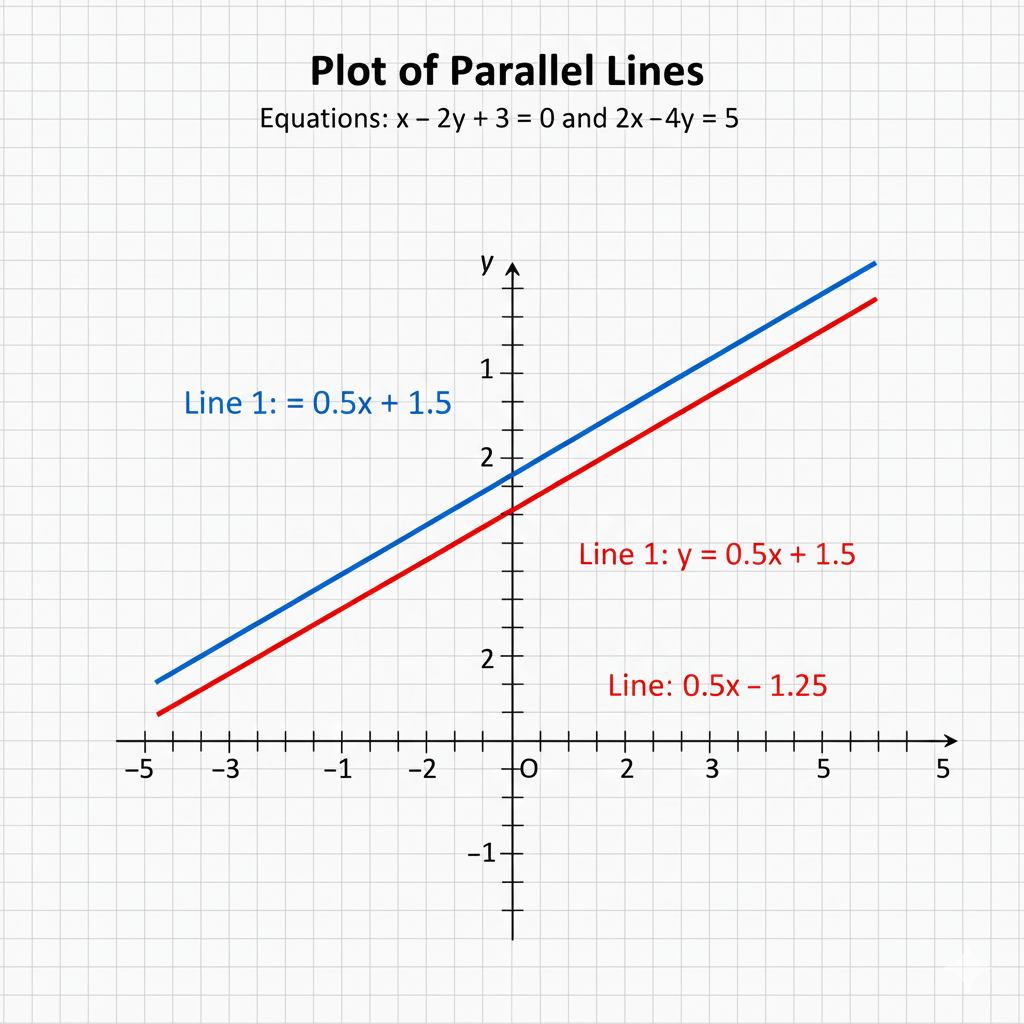
\includegraphics[width=\columnwidth]{figs/python_plot.png} 
\caption*{Plot of the curves}
\label*{Fig1}
\end{figure}


\end{document}
